
\chapter*{Introduction}   \addcontentsline{toc}{chapter}{Introduction} \label{intro}

The tessellation of surfaces and solids into complexes of small elements such as triangles, quadrilaterals, tetrahedra or hexahedra is one of the major
ingredients for many computational algorithms. Applications range from rendering, most notably in computer games, to computational science, in particular for the numerical solution of partial differential equations on complex domains for the study of physical phenomena. These various areas lead to a broad range of different requirements on a mesh library, which certainly cannot be fulfilled by a single, predetermined datastructure. Unlike other mesh libraries, {\ViennaGrid} provides the abililty to easily adjust the internal representation of meshes, while providing a uniform interface for the storage and access of data on mesh elements as well as STL-compatible iteration over such elements.

As example, consider the basic building block of triangular meshes, a triangle: The three vertices fully define the shape of the triangle, the edges can be derived from vertices if a common reference orientation of the triangles is provided. Depending on the underlying algorithm, edges of the triangle may or may not be of interest:
\begin{itemize}
 \item Consider a class \lstinline|triangle|, holding the three vertices only. A triangular mesh is then some array or list of \lstinline|triangle|s and an algorithm \texttt{algo1} working only on vertices on a per-cell basis can be executed efficiently. An example for such an algorithm is the assembly of a linear, nodal finite element method.

 \item An \texttt{algo2} may need to have global edge information available, i.e.~only one instance of an interfacing edge of two triangles should exist in an explicit manner.
       Thus, storing the edges globally in the domain will allow the use of \texttt{algo2}, but will at the same time introduce unnecessary edge information for \texttt{algo1}. Finite volume schemes can be seen as an example for this second type of algorithms.

 \item A third algorithm \texttt{algo3} may need global edge information, as well as information about the local orientation of edges with respect to each triangular cell.
      In such a case it may be preferred to additionally store mappings from global orientations to local orientations of the edges on each triangle if fast execution is desired.
      Such an additional storage of orientations will render the datastructure well suited for \texttt{algo3}, but less suited for \texttt{algo1} and \texttt{algo2}.
      An example for such a third type of algorithm are to some extent high-order finite element methods.
\end{itemize}
The situation for tetrahedral meshes is even more complicated, because additional orientation issues of shared facets come into play.

\begin{figure}[bt]
 \centering
\mbox{
\subfigure[Store only vertices globally, do not store edges.]{
 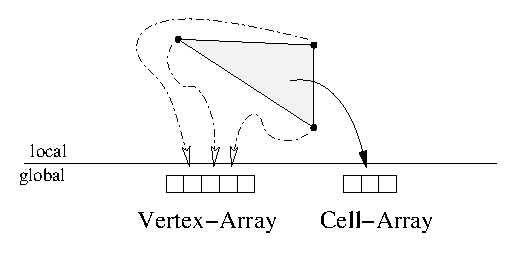
\includegraphics[scale=0.9]{figures/storage-vglob-cglob}
\label{subfig:storage-vglob-cglob}
} \hspace{0.5cm}
\subfigure[Store vertices and edges globally.]{
 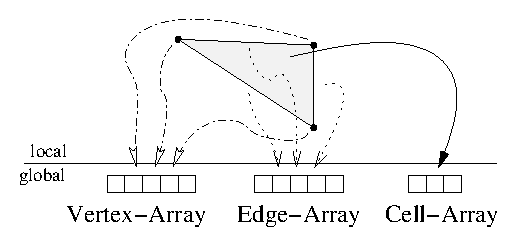
\includegraphics[scale=0.9]{figures/storage-vglob-eglob-cglob}
\label{subfig:storage-vglob-eglob-cglob}
} }
 \caption{Two storage schemes for a triangle and the underlying triangular mesh datastructure.}
 \label{fig:storage-schemes-triangle}
\end{figure}

The aim of {\ViennaGrid} is to be highly customizable such that all three algorithms outlined above can be supported with an optimal data layout. In particular, {\ViennaGrid} allows for a convenient specification of the storage of elements, in particular which boundary elements are stored inside the domain as well as which topological information is stored on each element. After a brief introduction into the nomenclature used in this manual in Chapter \ref{chap:entities}, the configuration of the data storage layout is explained in Chapter \ref{chap:domainconfig}, and the basic steps required to fill a mesh with cells is explained in Chapter \ref{chap:domainsetup}.

In addition to a high flexibility with respect to the underlying data structures, {\ViennaGrid} provides STL-compatible iterators and access to sub-elements of a mesh, cf.~Chapter \ref{chap:iterators}. This allows to write generic code that is a-priori independent of the underlying spatial dimension. In particular, a single implementation for algorithms operating in multiple dimensions and using different mesh types (triangular, hexahedral, etc.) can be obtained.

One of the strengths of {\ViennaGrid} is the generic facility provided for storing arbitrary quantities on a mesh, cf.~Chapter \ref{chap:data}. This is achieved by the use of the special purpose library {\ViennaData} \cite{ViennaData}, providing maximum flexibility for the user.

A typical requirement for a meshing library is mesh refinement. This is in particular of interest for computational science, where singularities near corners need to be resolved sufficiently well. {\ViennaGrid} provides both uniform and adaptive refinement algorithms, cf.~Chapter \ref{chap:algorithms}, where also other geometric algorithms such as Voronoi information is covered.

Input/Output facilities are discussed in Chapter \ref{chap:io}. Some of the library internals are discussed in Chapter \ref{chap:internals} and design decisions are outlined in Chapter \ref{chap:design}.

There are of course a number of other free software libraries having functional overlap with {\ViennaGrid}. We give a brief discussion of the pros and cons of selected libraries in the following. This should allow potential users of our library to get a better feeling of what to expect and what not to expect from {\ViennaGrid}. We have carefully checked the documentation of each project, but clearly cannot guarantee that all information is fully accurate.
\begin{itemize}
  \item \textbf{CGAL} \cite{CGAL}: The focus of the Computational Geometry Algorithms Library (\texttt{CGAL}) is on geometrical algorithms such as the computation of convex hulls of point sets. It offers a mesh generation facility and provides iterators over cell vertices. However, the storage of quantities and the convenient traversal of mesh elements is not provided.

  \item \textbf{DUNE} \cite{DUNE}: \texttt{DUNE} follows a similar approach for the generic representation of meshes. It provides support for conforming and non-conforming grids, as well as support for parallel and distributed meshes. However, unlike {\ViennaGrid}, we could not find any mechanism providing a convenient means to store data on mesh elements (users are essentially required to handle their data themselves), and for the customization about the internal storage of mesh elements.

  \item \textbf{GrAL} \cite{GrAL}: The Grid Algorithms library (\texttt{GrAL}) provides mesh data structured and algorithms operating on them. A number of principles used in {\ViennaGrid} such as $n$-\textit{cells} already show up in \texttt{GrAL} as $k$-\textit{Elements}. The library does not provide any facility to store data on mesh elements. Mesh refinement is also not provided.

  \item \textbf{libmesh} \cite{libmesh}: The \texttt{libmesh} library is not only a mesh library, but also a framework for numerical simulations. Since {\ViennaGrid} is designed to be as general as possible without prematurely restricting to a particular application, we only compare the parts in \texttt{libmesh} related to mesh handling. \texttt{libmesh} supports one-, two- and three-dimensional meshes and also allows to generate meshes for simple domains. Iterations over elements of a mesh are carried out in a runtime manner, thus causing potential overhead. One of the strengths of \texttt{libmesh} is the support for mesh refinement and parallel computations. Support for user-defined data on mesh elements is also provided.

  \item \textbf{OpenMesh} \cite{OpenMesh}: \texttt{OpenMesh} provides a generic datastructure for representing and manipulating polygonal meshes. The main goals are flexibility, efficiency and easy-to-use. Similar to {\ViennaGrid}, generic programming paradigms are used. \texttt{OpenMesh} allows to store custom data of arbitrary type on mesh elements, but it seems to rely on potentially slow string comparisons at run-time to retrieve the data. Moreover, \texttt{OpenMesh} is specifically designed for surface (i.e.~non-volumetric) meshes, and thus only the concepts of vertices, edges and faces are used.

  \item \textbf{trimesh2} \cite{trimesh2}: \texttt{trimesh2} is a C++ library that is particularly designed for triangular meshes in 3D only. It explicitly targets efficiency, possibly at the expense of some generality. We could not find further information for a comparison with {\ViennaGrid} from the documentation provided.

  \item \textbf{VCGlib} \cite{VCGlib}: \texttt{VCGlib} processes triangular and tetrahedral meshes. Similar to \texttt{OpenMesh}, \texttt{VCGlib} uses the concepts of vertices, edges and faces only, so the processing of volume meshes is hampered. Again similar to \texttt{OpenMesh}, the provided facility to store data on mesh elements relies on potentially slow string comparisons.
\end{itemize}




